\documentclass[border=5pt,tikz]{standalone}
\usepackage{tikz}
\usepackage{amsmath}
\usepackage{amssymb}
\usepackage{ctex}
\usetikzlibrary{matrix, calc, positioning}
\usepackage{pgfplots}
\pgfplotsset{compat=1.18}

\begin{document}

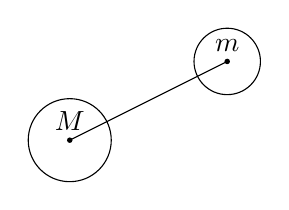
\begin{tikzpicture}
	\draw (0,0) circle [radius = 15pt] node[above] {$M$}
	(2,1) circle [radius=12pt] node[above] {$m$};
	\fill (0,0) circle[radius=1pt]
	(2,1) circle[radius=1pt];
	\draw (0,0) -- (2,1);

\end{tikzpicture}

\end{document}
